\documentclass[fleqn,10pt,lineno]{wlpeerj}\usepackage[]{graphicx}\usepackage[]{color}
%% maxwidth is the original width if it is less than linewidth
%% otherwise use linewidth (to make sure the graphics do not exceed the margin)
\makeatletter
\def\maxwidth{ %
  \ifdim\Gin@nat@width>\linewidth
    \linewidth
  \else
    \Gin@nat@width
  \fi
}
\makeatother

\definecolor{fgcolor}{rgb}{0.345, 0.345, 0.345}
\newcommand{\hlnum}[1]{\textcolor[rgb]{0.686,0.059,0.569}{#1}}%
\newcommand{\hlstr}[1]{\textcolor[rgb]{0.192,0.494,0.8}{#1}}%
\newcommand{\hlcom}[1]{\textcolor[rgb]{0.678,0.584,0.686}{\textit{#1}}}%
\newcommand{\hlopt}[1]{\textcolor[rgb]{0,0,0}{#1}}%
\newcommand{\hlstd}[1]{\textcolor[rgb]{0.345,0.345,0.345}{#1}}%
\newcommand{\hlkwa}[1]{\textcolor[rgb]{0.161,0.373,0.58}{\textbf{#1}}}%
\newcommand{\hlkwb}[1]{\textcolor[rgb]{0.69,0.353,0.396}{#1}}%
\newcommand{\hlkwc}[1]{\textcolor[rgb]{0.333,0.667,0.333}{#1}}%
\newcommand{\hlkwd}[1]{\textcolor[rgb]{0.737,0.353,0.396}{\textbf{#1}}}%
\let\hlipl\hlkwb

\usepackage{framed}
\makeatletter
\newenvironment{kframe}{%
 \def\at@end@of@kframe{}%
 \ifinner\ifhmode%
  \def\at@end@of@kframe{\end{minipage}}%
  \begin{minipage}{\columnwidth}%
 \fi\fi%
 \def\FrameCommand##1{\hskip\@totalleftmargin \hskip-\fboxsep
 \colorbox{shadecolor}{##1}\hskip-\fboxsep
     % There is no \\@totalrightmargin, so:
     \hskip-\linewidth \hskip-\@totalleftmargin \hskip\columnwidth}%
 \MakeFramed {\advance\hsize-\width
   \@totalleftmargin\z@ \linewidth\hsize
   \@setminipage}}%
 {\par\unskip\endMakeFramed%
 \at@end@of@kframe}
\makeatother

\definecolor{shadecolor}{rgb}{.97, .97, .97}
\definecolor{messagecolor}{rgb}{0, 0, 0}
\definecolor{warningcolor}{rgb}{1, 0, 1}
\definecolor{errorcolor}{rgb}{1, 0, 0}
\newenvironment{knitrout}{}{} % an empty environment to be redefined in TeX

\usepackage{alltt} % for journal submissions
\usepackage{hyperref}
% \documentclass[fleqn,10pt]{wlpeerj} % for preprint submissions

\title{Using metagenomic methods to detect organismal contaminants in microbial materials.}

\author[1]{Nathan D. Olson}
\author[1]{Justin Zook}
\author[1]{Jayne Morrow}
\author[1]{Nancy Lin}
\affil[1]{Material Measurement Laboratory, National Institute of Standards and Technology}

\keywords{Biodetection, Microbial Material, Reference Material, Purity, Bioinformatics}

\begin{abstract}
\textbf{TODO}
% - basic introduction
% - more detailed background
% - general problem
% - main result summary
% - explanation of what main result reveals
% - general context
% - broader perspective

\end{abstract}
\IfFileExists{upquote.sty}{\usepackage{upquote}}{}
\begin{document}



\flushbottom
\maketitle
\thispagestyle{empty}

\section*{Introduction}
Shotgun metagenomic sequencing is used to characterize environmental samples and detect pathogens in complex samples.
The same method can also be used to detect contaminants in microbial materials, cell cultures and genomic DNA from clinical or environmental isolates.
Microbial materials free of contaminants are needed for biodetection assay validation \citep{Ieven2013,International2011} and basic research using model systems \citep{Shrestha2013}.
Current methods for detecting contaminants in microbial materials use traditional methods such as culture, microscopy and polymerase chain reaction (PCR) (REF). 
Culture and microscopy based methods are not appropriate for genomic DNA materials and assumes the contaminants are phenotypically distinct from the material isolate it is contaminanting. 
While, PCR based methods can be used to detect contaminants in genomic DNA, the method is limited as contaminant detection assays are contaminant specific and not ammenable to high-throughput applications \citep{heck2016evaluating,Marron2013}. 
In contrast to these methods, shotgun metagenomic methods can be used to detect contaminants in both cell cultures and genomic DNA materials and only require that the contaminant is genotypically differentiable from the material strain. 

Shotgun metagenomics consists of two main steps, whole genome sequencing of genomic DNA, and analyzing the resulting sequencing data, most commonly using a taxonommic assignment algorithm \citep{Thomas2012}.
For genomic DNA material, the material itself can be sequenced, whereas the genomic DNA must be extracted from from cell cultures prior to sequencing. 
After sequencing a taxonomic assignment algorithm is used to characterize the sequencing data. 
There are a number of different types of classification algorithms with varying classification accuracy and computational performance \citep{Bazinet2012,menzel2016fast}.
All methods require a reference database for classification.
In order to detect a contaminant within a microbial material, the contaminant or an organism more closely related to the contaminant than the material must be present in the database. 
As taxonomic classification algorithms are constantly improving, reference databases are expanding, and the cost of sequencing drops, shotgun metagenomic sequencing provides an alternative to current methods for detecting contaminants in microbial materials.

In this work, we present the results of a proof of concept study evaluating the suitability of whole genome sequencing data combined with a taxonomic assignment algorithm for detecting organismal contaminants in microbial materials.
We first provide a baseline assessment of the method using simulated sequencing data from single organisms to characterize the types of false positive contaminants the method may report.
Then, evaluate the method's ability to detect organismal contaminants in microbial material strains using sequencing data simulated to replicate microbial materials with different organismal contaminants at a range of concentrations.

\section*{Methods}
Simulated whole genome sequence data was used to evaluate the suitability of using whole genome sequence data and metagenomic taxonomic classification methods for detecting organismal contaminants in microbial materials.
Simulated data from single genomes was used to characterize the rate at which the method correctly classifies reads as the test material.
To characterize the method's ability to detect contaminants, simulated contaminant datasets comprised of pairwise combinations of single genomes spiked with a defined proportions of contaminant reads, reads simulated from a different genome.

To best approximate real sequencing data reads were simulated using an empirical error model and insert size distribution.
Whole genome sequencing data was simulated using the ART sequencing read simulator \citep{Huang2012}.
Reads were simulated with ART simulator using the Illumina MiSeq error model for 2 $\times$ 230 base pair (bp) paired end reads with an insert size of 690 $\pm$ 10 bp (average $\pm$ standard deviation) and 20 X mean coverage.
The insert size parameters were defined based on the observed average and standard deviation insert size of the NIST RM8375-MG002 MiSeq sequencing data \citep{olson2016pepr}.

The taxonomic composition of simulated datasest was assessed using the Pathoscope sequence taxonomic classifier \citep{Francis2013}.
Pathoscope was selected as it combines the use of a large reference database reducing potential biases due to contaminant sequences not present in the database and efficient whole genome read mapping algorithms.
This method uses an expectation maximization algorithm where the sequence data are first mapped to a database comprised of all sequence data in the Genbank nt database.
Then, through an iterative process, it re-assigns ambiguously mapped reads based on the proportion of reads mapped unambigously to individual taxa in the database.
The Pathoscope 2.0 taxonomic read classification pipeline has three steps; (1) PathoQC - read quality filtering and trimming using the PRINSEQ algorithm \citep{schmieder2011quality}, (2) PathoMap - mapping reads to a reference database using the bowtie2 algorithm \citep{Langmead2012}, (3) PathoID - expectation-maximization classification algorithm.
The annotated Genbank nt database provided by the PathoScope developers was used as the reference database (\url{ftp://pathoscope.bumc.bu.edu/data/nt\_ti.fa.gz}).

\subsection*{Single Genome - Baseline Assessment}
Simulated sequencing data from individual genomes was used to characterize the false positive contaminants reported by Pathoscope. 
Sequence data was simulated for 406 strains, from 9 genera (Table \ref{tab:single_org}).
We will refer to the genome used to generate the reads as the target genome.
The genomes included in the simulation study were limited to the number of closed genomes in the Genbank database (\url{http://www.ncbi.nlm.nih.gov/genbank/}, accessed 10/18/2013) belonging to the genera of interest (Table \ref{tab:single_org}).
Due to the large number of closed genomes from the genera \textit{Bacillus}, \textit{Escherichia}, and \textit{Salmonella}, genomes from these genera were limited to the species \textit{Bacillus cereus}, \textit{Escherichia coli}, and \textit{Salmonella enterica}.
The taxononomic hierarchy for the target genome and simulated read assignment match levels were determined using the R package, Taxize \citep{TaxizeArticle,TaxizeManual}.

\subsection*{Simulated Contaminants}
Simulated contaminated datasets were used to evaluate how contaminant dection varied by material and contaminant strain over a range of contaminant concentrations.
Representative genomes for 8 of the 9 genus were used to generate the simulated contaminant datasets (Table \ref{tab:contam_table}).
An \textit{Escherichia coli} strain was selected as a representative of both  and \textit{Shigella} as the genus \textit{Shigella} phylogenetically resides within the species \textit{Eschericha coli} \citep{lan2002escherichia}.
For each pairwise combination of representative genomes the simulated contaminant dataset was comprised of a randomly selected subset of reads from the target and contaminant simulated single genome sequence dataset.
The simulated datasets were subsampled at defined proportions with $p$ representing the proportion of reads from the contaminant single genome dataset subsampled and $1-p$ the proportion of reads from the target genome simulated dataset.
\textit{Make Sure to Revise for Clarity - Maybe include a figure/diagram.}
A 10 fold range of contaminant proportions were simulated with $p$ ranging from $0.1$ to $10^{-8}$, resulting in 512 simulated contaminant datasets.
This approach simulates the proportions of cells in a contaminanted material and not the amount of DNA, assuming unbiased DNA extraction.

To generate the simulated contaminant datasets single organism simulated datasets were first generated for the 8 representative genomes using the same methods as used in baseline assessment.
The resulting simulated sequencing data was first processed using the PathoQC and PathoMap steps in the Pathoscope pipeline.
The output from the PathoMap step (sam file, sequence alignment file \url{https://samtools.github.io/hts-specs/SAMv1.pdf}) for the material and contaminant datasets were subsampled as described above then combined. 
The resulting sam file was processed by PathoID, the third step in the Pathoscope pipeline.
Subsampling the sam files instead of the simulated sequence files greatly reduces the computational cost of the analysis as the simulated reads were only processed by the first two steps in Pathoscope pipeline once rather then for every simulated contaminant dataset.


\subsection*{Bioinformatic Pipeline}
To facilitate repeatability and transparency, a Docker (\url{www.docker.com}) container is available with installed pipeline dependencies (\url{www.registry.hub.docker.com/u/natedolson/docker-pathoscope/}).
The script used to run the simulations are available at \url{https://github.com/nate-d-olson/genomic_purity}.
Additionally, seed numbers for the random number generator were randomly assigned and recorded for each dataset so that the same simulated datasets could be regenerated.
Pathoscope results were processed using the statistical programing language R \citep{R}, and intermediate analysis and data summaries were organized using ProjectTemplate \citep{ProjectTemplate} and archived in a github repository (\url{https://github.com/nate-d-olson/genomic_purity_analysis}) along with the source file for this manuscript.

\section*{Results}

\subsection*{Single Genome - Baselines Assessment}
We first assessed baseline performance of the proposed method for detecting organismal contaminants in microbial materials. 
Our analysis included taxonomic classification results for simulated sequencing data  from 388 genomes, representing 9 different genera (Table \ref{tab:single_org}). 
For 105 out of 388 genomes, Pathoscope estimated that 99\% of the material was the same species as the genome the sequencing data was simulated from (Fig. \ref{fig:species_prop}). 
The estimated proportion of the material identified as the correct species varied by genus, with none of the \textit{Shigella} genomes and five of the 49 \textit{Staphylococcus} genomes having proportions greater than 0.9. \textit{Shigella} and \textit{Staphlyococcus} along with \textit{Escherichia} represent 87 of the 105 genomes with a less than 0.99 estimated match proportions at the species level. Excluding \textit{Shigella}, \textit{Escherichia}, and \textit{Staphylococcus} the median estimated proportion matching at the species level or higher is  0.9995. The low species level match proportions were due to false positive contaminants as the input sequencing data were simulated from individual genome sequences.

% latex table generated in R 3.3.1 by xtable 1.8-2 package
% Tue Oct 11 12:08:31 2016
\begin{table}[ht]
\centering
\begin{tabular}{lrl}
  \hline
Genus & N & Genome Size (Mb) \\ 
  \hline
\textit{Bacillus} &  76 & 5.05 (3.07-7.59) \\ 
  \textit{Escherichia} &  62 & 5.11 (3.98-5.86) \\ 
  \textit{Pseudomonas} &  57 & 6.18 (4.17-7.01) \\ 
  \textit{Staphylococcus} &  49 & 2.82 (2.69-3.08) \\ 
  \textit{Salmonella} &  44 & 4.88 (4.46-5.27) \\ 
  \textit{Listeria} &  39 & 2.97 (2.78-3.11) \\ 
  \textit{Clostridium} &  32 & 4.02 (2.55-6.67) \\ 
  \textit{Yersinia} &  19 & 4.73 (4.62-4.94) \\ 
  \textit{Francisella} &  18 & 1.89 (1.85-2.05) \\ 
  \textit{Shigella} &  10 & 4.74 (4.48-5.22) \\ 
   \hline
\end{tabular}
\caption{Breakdown of the number of genomes by genus used to generate single genome simulated datasets. N indicates the number of genomes, and Genome Size is presented as the median and range (minimum to maximum) genome size} 
\label{tab:single_org}
\end{table}


\begin{knitrout}
\definecolor{shadecolor}{rgb}{0.969, 0.969, 0.969}\color{fgcolor}\begin{figure}
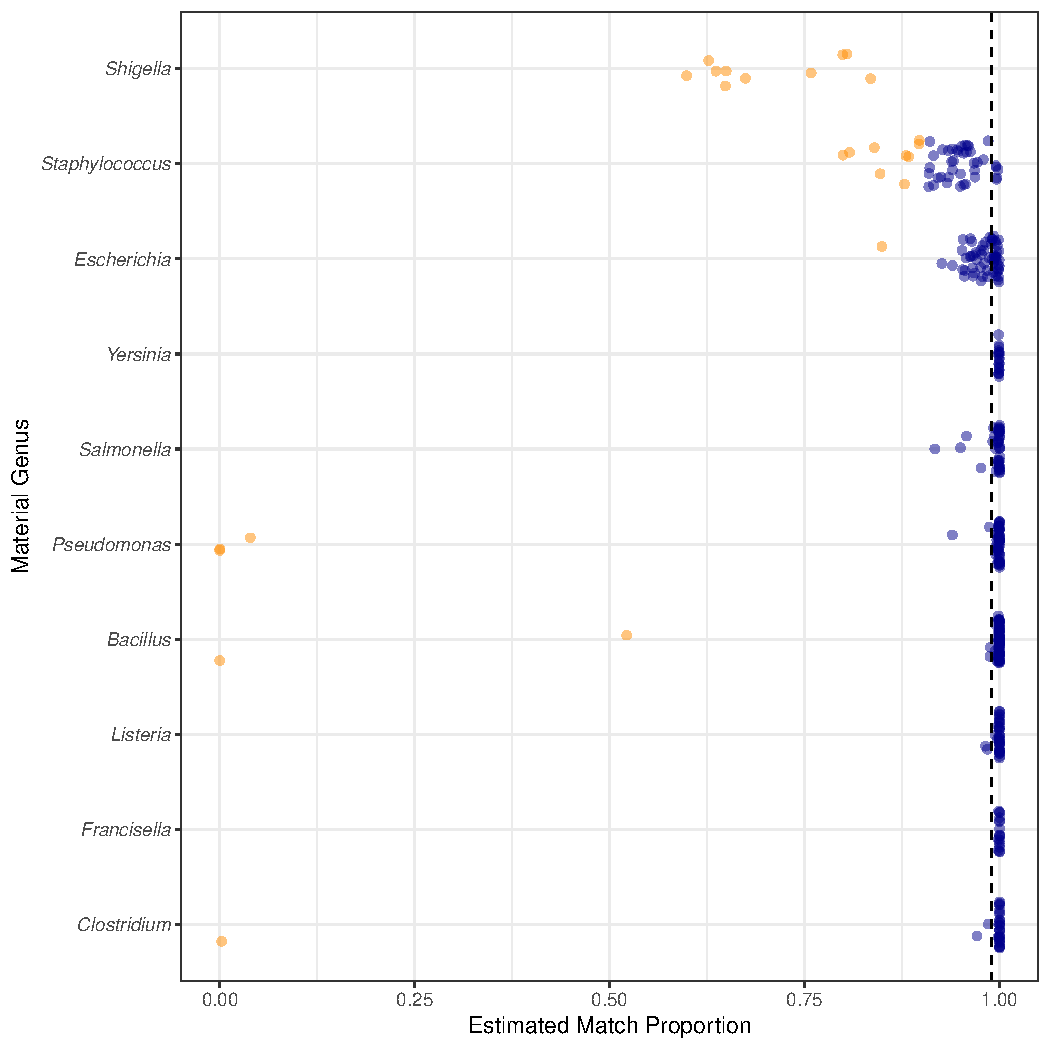
\includegraphics[width=\maxwidth]{figure/species_prop-1} \caption[Species level estimated match proportion varies by material genus]{Species level estimated match proportion varies by material genus. The proportion of the material, simulated sequence data from individual genomes, was estimated by Pathoscope. The estimated match proportion is the total proportion of the material with taxonomic assignments to the genome species, subspecies, strain, or isolate levels. The vertical dashed line indicates the 0.99 match proportion. Orange points are genomes with species level match proportions less than 0.90 and blue points greater than 0.90}\label{fig:species_prop}
\end{figure}


\end{knitrout}

We characterized the false postive contaminants responsible for the genera \textit{Shigella}, \textit{Escherichia}, and \textit{Staphylococcus}, as well as genomes of other genera with species match proportions less than 0.9. 
The false positive contmainants were grouped into three types, taxonomic ambiguities, phage, and method artifacts.  
Taxonomic ambiguities were defined as contaminants with highly similar genome sequences to the material genome sequence but taxonomically classified as different species. 
For example the low match percentage for \textit{Clostridium autoethanogenum} strain DSM10061 was due to  \textit{Clostridium ljungdahlii} strain DSM13528 assigned the top proportion (\textbf{VALUE}) instead of \textit{C. autoenthanogenum}. 
Similarly, \textit{Escherichia coli} strain UMNK88 low match, due to two bacteria in the same family as \textit{E. coli}, 
Enterobacteriaceae, \textit{Providencia stuartii} and \textit{Salmonella enterica} subsp. enterica serovar Heidelberg with estimated proportions of \textbf{VALUE} and \textbf{VALUE} respectively. 
Taxonomic ambiguities can be due to a species being incorrectly assigned to the wrong taxonomic group for example the \textit{Bacillus} genome with species match proportion close to zero, \textit{Bacillus infantis} string NRRL B 14911. 
While the \textit{B. infantis} strain was originally classified as \textit{Bacillus}, the species is phylogenetically distinct from other members of the genus \citep{ko2006bacillus}. 
Taxonomic ambiguities are at least partially responsible for the low species level match proportions for  \textit{Shigella} and \textit{Escherichia}, as \textit{Shigella} is not phylogenetically distinct from \textit{E. coli}(\textbf{REF}).
When including matches to \textit{E. coli} as species level matches, the median match proportions increase from 0.66 to 0.92. 
Though considerably higher, this match proportion is still low relative to the other genera \textbf{INCLUDE VALUE DIFFERENCE}.  

%%\textbf{NOTE Table with median species level match proportions}. 

\begin{knitrout}
\definecolor{shadecolor}{rgb}{0.969, 0.969, 0.969}\color{fgcolor}\begin{figure}
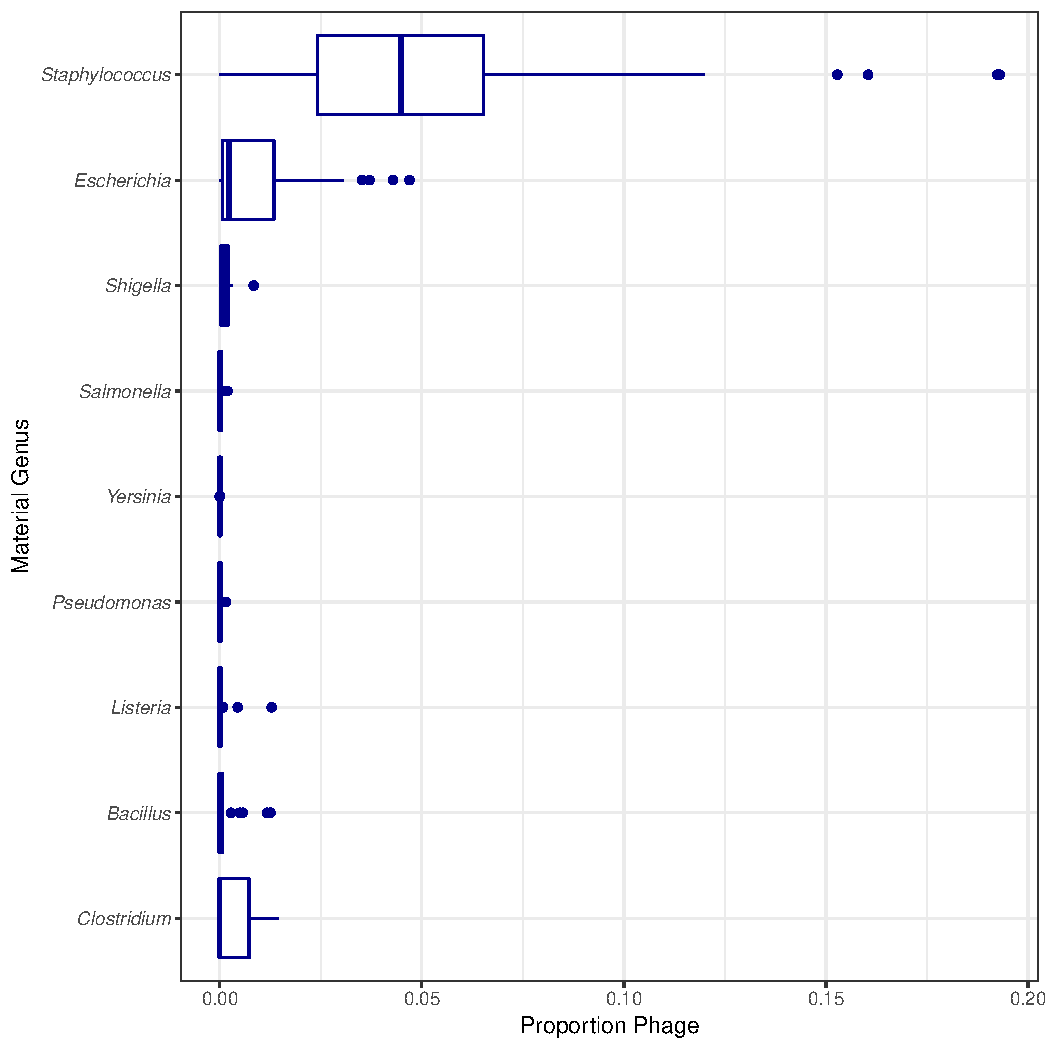
\includegraphics[width=\maxwidth]{figure/phage_prop-1} \caption[Estimated proportion of phage in the simulated single genome datasets by genera]{Estimated proportion of phage in the simulated single genome datasets by genera.}\label{fig:phage_prop}
\end{figure}


\end{knitrout}

Phage, the second type of false positive contaminant, were reported by Pathoscope as present in varing proportions for genomes from all 9 genera investigated (Fig. \ref{fig:phage_prop}). 
Most noteably, low proportions of species level matches for \textit{E. coli} and \textit{Staphylococcus} is partly due to relatively higher proportions of matches to phage, compared to the other genera investigated (Fig. \ref{fig:phage_prop}). 
All of the false postive phage contmaninants were specific to the taxonomy of the genome the sequence data was simulated from. 
The phage contaminants may represent errors in the database, where sequence data from the host organisms genome is missassembled into the phage genome, or genomic sequence is shared between the phage and the host, such as CRISPR, and lysogenic phage (REF).  

\textbf{Method Artifacts}
The third type of false positive contaminant, are method artifacts. Method artifact false positive contaminants are defined as false positives due to missclassified or unclassified sequences in the database, genome assemblies in the database including sequence data from organismal or reagent contaminants, and errors associated with the classification algorithm. 
\textit{Bacillus subtilis} BEST7613 genome had low estimated species level match proportion due to \textit{Synechocystis} sp. PCC 6803 substr. PCC-P being estimated as comprising 47\% of the material  \citep{kanesaki2012identification}. \textit{Synechocystis} is in a different phylum compared to \textit{Bacillus}, cyanobacteria versus firmicutes. 
The high match proportion is not due to taxonomic ambuguities but potentially an error in the database. 
Low species level match proportions can also be due to the database containing unclassified sequence data for organisms highly similar to the material genome. 
For example the low match proportion for \textit{Pseudomonas} strain FGI182 was due to matches to unclassified bacteria, bacterium 142412, and unclassified $Pseudomonas$ species, $Pseudomonas$ sp. HF-1.  
The eukaryotic false positive contaminants are likely either due to similarities between the genome sequences or errors in the assembly \textbf{REF}. 
Plasmids and vectors are common used molecular biology tools and well known contmainants of sequencing data (REF).
The plasmids and vectors identified as false positive contaminants due to errors in the genome assemblies where artifacts of the sequencing process were not properly removed from the sequencing data prior to assembly. 
Alternatively, the misclassification could be due to high similarity between the genome sequence the reads were simulated from and the plasmid and vector sequence which is not unexpected as most plasmid and vectors have microbial origins (REF). 
The low species proportion of species level matches for \textit{Pseudomonas} strain TKP was likely due to both missclassified sequences (\textit{Thioalkalivibrio sulfidophilus} strain HL-EbGr7 match proportion 0.0648), and contminanted genome sequences in the database (wheat - \textit{Triticum aestivum} match proportion 0.087).
Errors associated with the classification algorithm are likely resposible for low species level match path proportion for \textit{Pseudomonas} strain VLB120 is likely due to errors in the database as $2.6x10^{-3}$ of the matches assigned to the unrelated species \textit{Xanthomonas} sp. W17. 
The representative database sequence is ~9 kb (https://www.ncbi.nlm.nih.gov/nuccore/710572), the Pathoscope expectation maximization step include a length normalization step which is likely responsible for the classification error. 

\subsection*{Simulated Contaminants - Detection Assessment}
% latex table generated in R 3.3.1 by xtable 1.8-2 package
% Tue Oct 11 12:08:31 2016
\begin{table}[ht]
\centering
\scalebox{0.65}{
\begin{tabular}{lrllll}
  \hline
Representative Strain & Species & C Mb & C Acc & P Mb & P Acc \\ 
  \hline
Bacillus anthracis str. Ames & 1.00 & 5.23 & AE016879.1 &  &  \\ 
  Clostridium botulinum A str. Hall & 1.00 & 3.76 & CP000727.1 &  &  \\ 
  Escherichia coli O157:H7 str. EC4115 & 0.98 & 5.57 & CP001164.1 & 0.13 & CP001163.1, CP001165.1 \\ 
  Francisella tularensis subsp. tularensis SCHU S4 & 1.00 & 1.89 & AJ749949.2 &  &  \\ 
  Pseudomonas aeruginosa PAO1 & 1.00 & 6.26 & AE004091.2 &  &  \\ 
  Salmonella enterica subsp. enterica serovar Typhimurium str. D23580 & 1.00 & 4.88 & FN424405.1 &  &  \\ 
  Staphylococcus aureus subsp. aureus ED133 & 0.98 & 2.83 & CP001996.1 &  &  \\ 
  Yersinia pestis CO92 & 1.00 & 4.65 & AL590842.1 & 0.18 & AL109969.1, AL117189.1, AL117211.1 \\ 
   \hline
\end{tabular}
}
\caption{Representative strains used in simulated contaminant datasets. Species indicates the proportion of the material assigned to the correct species. DNA size (Mb) and Genbank accession numbers (Acc) are indicated for chromosomes (C) and plasmids (P). Escherichia coli O157:H7 str. EC4115 and Yersinia pestis CO92 have two and three plasmids respectively.} 
\label{tab:contam_table}
\end{table}


%%TODO%% Italicize species names in table caption above

Next we evaluated how well contaminants were detected.
Using simulated sequencing data from individual genomes we generated contaminant datasets by combining subsets of simulatd data from two organisms at defined proportions,
with the larger proportion representing the microbial material and smaller proportion the contaminant.
We simulated contaminant datasets as pairwise combinations of representative genomes from 8 of the genera used in the baseline assessment section of the study (Table \ref{tab:contam_table}).
For all of the genomes selected for the detection assessment study, the estimated proportion of material assigned to the correct species was 0.98 (Table \ref{tab:contam_table}).

% latex table generated in R 3.3.1 by xtable 1.8-2 package
% Tue Oct 11 12:08:31 2016
\begin{table}[ht]
\centering
\scalebox{0.85}{
\begin{tabular}{lrrrrrrrr}
  \hline
contam\_label & Baci & Clos & Esch & Fran & Pseu & Salm & Stap & Yers \\ 
  \hline
Bacillus anthracis Ames &  & 1.0E-03 & 1.0E-08 & 1.0E-03 & 1.0E-03 & 1.0E-03 & 1.0E-03 & 1.0E-03 \\ 
  Clostridium botulinum A Hall & 1.0E-03 &  & 1.0E-03 & 1.0E-03 & 1.0E-03 & 1.0E-03 & 1.0E-03 & 1.0E-03 \\ 
  Escherichia coli O157 H7 EC4115 & 1.0E-03 & 1.0E-03 &  & 1.0E-03 & 1.0E-03 & 1.0E-03 & 1.0E-03 & 1.0E-08 \\ 
  Pseudomonas aeruginosa & 1.0E-04 & 1.0E-04 & 1.0E-04 & 1.0E-04 &  & 1.0E-04 & 1.0E-04 & 1.0E-04 \\ 
  Salmonella enterica serovar Typhimurium & 1.0E-03 & 1.0E-03 & 1.0E-03 & 1.0E-03 & 1.0E-03 &  & 1.0E-03 & 1.0E-08 \\ 
  Staphylococcus aureus ED133 & 1.0E-04 & 1.0E-04 & 1.0E-04 & 1.0E-04 & 1.0E-04 & 1.0E-04 &  & 1.0E-04 \\ 
  Yersinia pestis CO92 & 1.0E-01 & 1.0E-01 & 1.0E-01 & 1.0E-01 & 1.0E-01 & 1.0E-01 & 1.0E-01 &  \\ 
   \hline
\end{tabular}
}
\caption{Lowest proportion of contaminant in each pairwise combination of representative genomes detected.} 
\label{tab:contam_min_table}
\end{table}



The minimum contaminant proportion detected was $10 \times 10^{-3}$ and  $10 \times 10^{-4}$ for most pairwise comparisons with a few notable exceptions. 
When \textit{Yersina} was the simulated contaminant the minimum detected proportion was 0.1 for all material strains (Table \ref{tab:contam_min_table}).
Conversely, contaminants were detected at lower proportions, $10 \times 10^{-8}$, when \textit{Yersinia} was contaminated with \textit{E. coli} as well as when \textit{S. enterica} and \textit{E. coli} contaminated with \textit{B. anthracis}.  

%%TODO%% Statement about reasoning for why consistency and outliers


\begin{knitrout}
\definecolor{shadecolor}{rgb}{0.969, 0.969, 0.969}\color{fgcolor}\begin{figure}
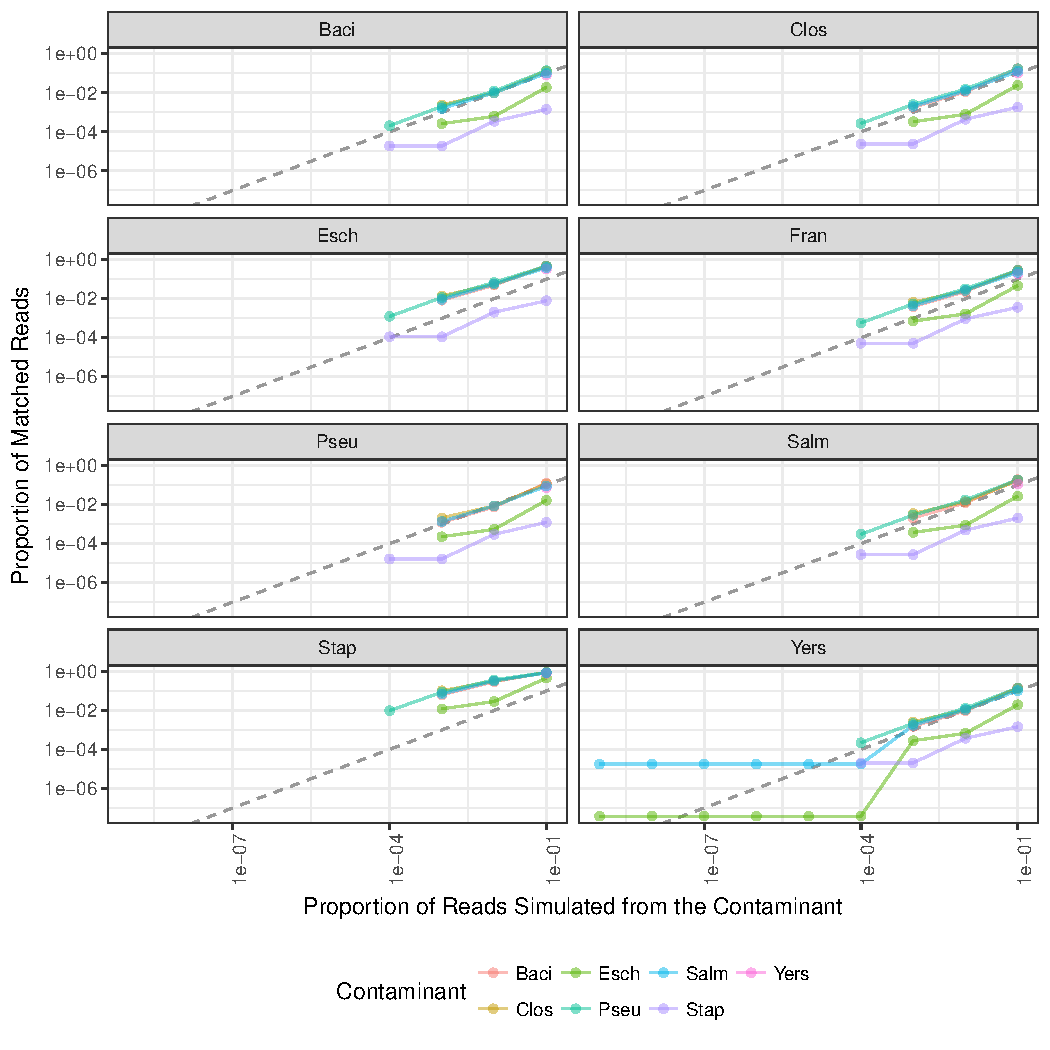
\includegraphics[width=\maxwidth]{figure/contam_fig-1} \caption[Relationship between the proportion of contaminant reads simulated per dataset and the proportion of reads matched to the contaminant genus]{Relationship between the proportion of contaminant reads simulated per dataset and the proportion of reads matched to the contaminant genus.}\label{fig:contam_fig}
\end{figure}


\end{knitrout}

\begin{knitrout}
\definecolor{shadecolor}{rgb}{0.969, 0.969, 0.969}\color{fgcolor}\begin{figure}
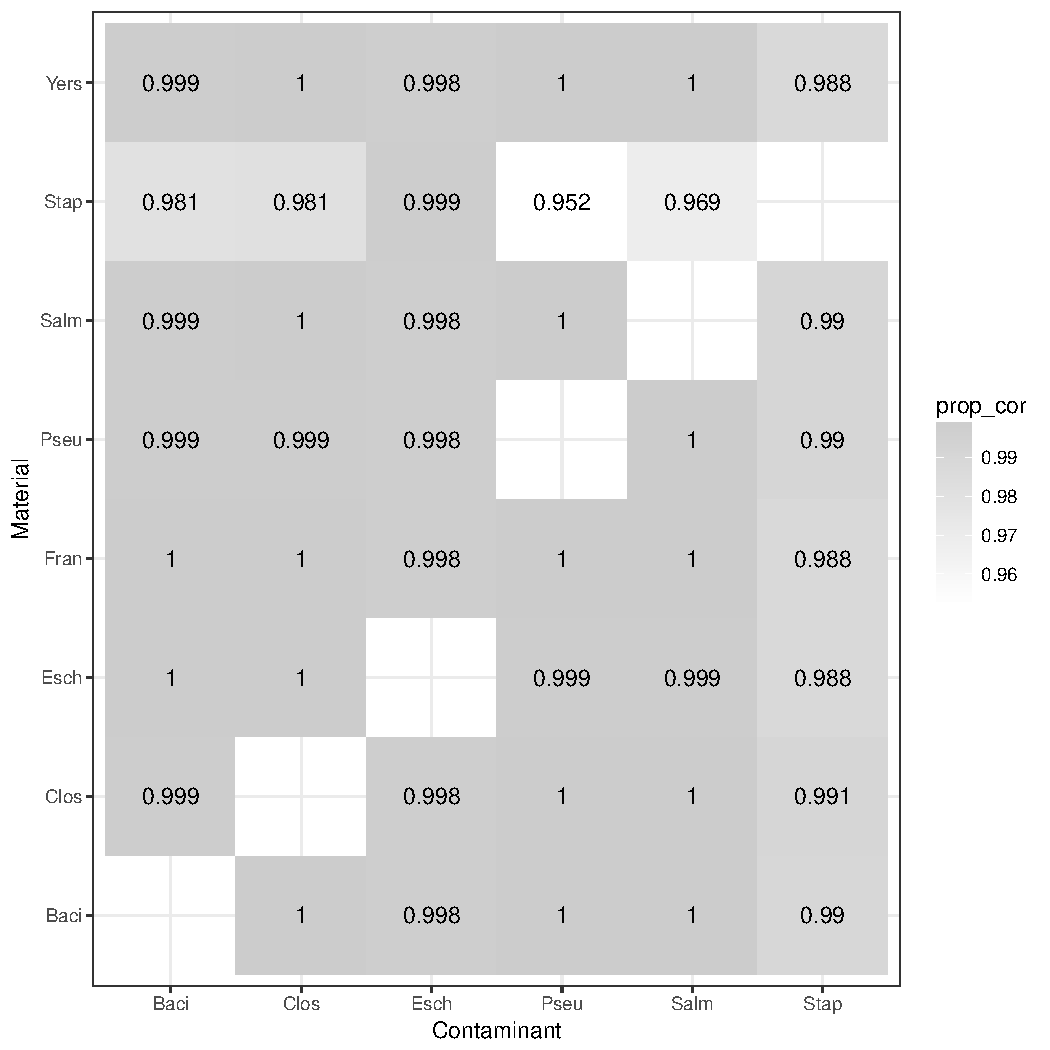
\includegraphics[width=\maxwidth]{figure/contam_corr-1} \caption[Pearson correlation coefficients for estimated and true contaminant proportions]{Pearson correlation coefficients for estimated and true contaminant proportions.}\label{fig:contam_corr}
\end{figure}


\end{knitrout}


\begin{knitrout}
\definecolor{shadecolor}{rgb}{0.969, 0.969, 0.969}\color{fgcolor}\begin{figure}
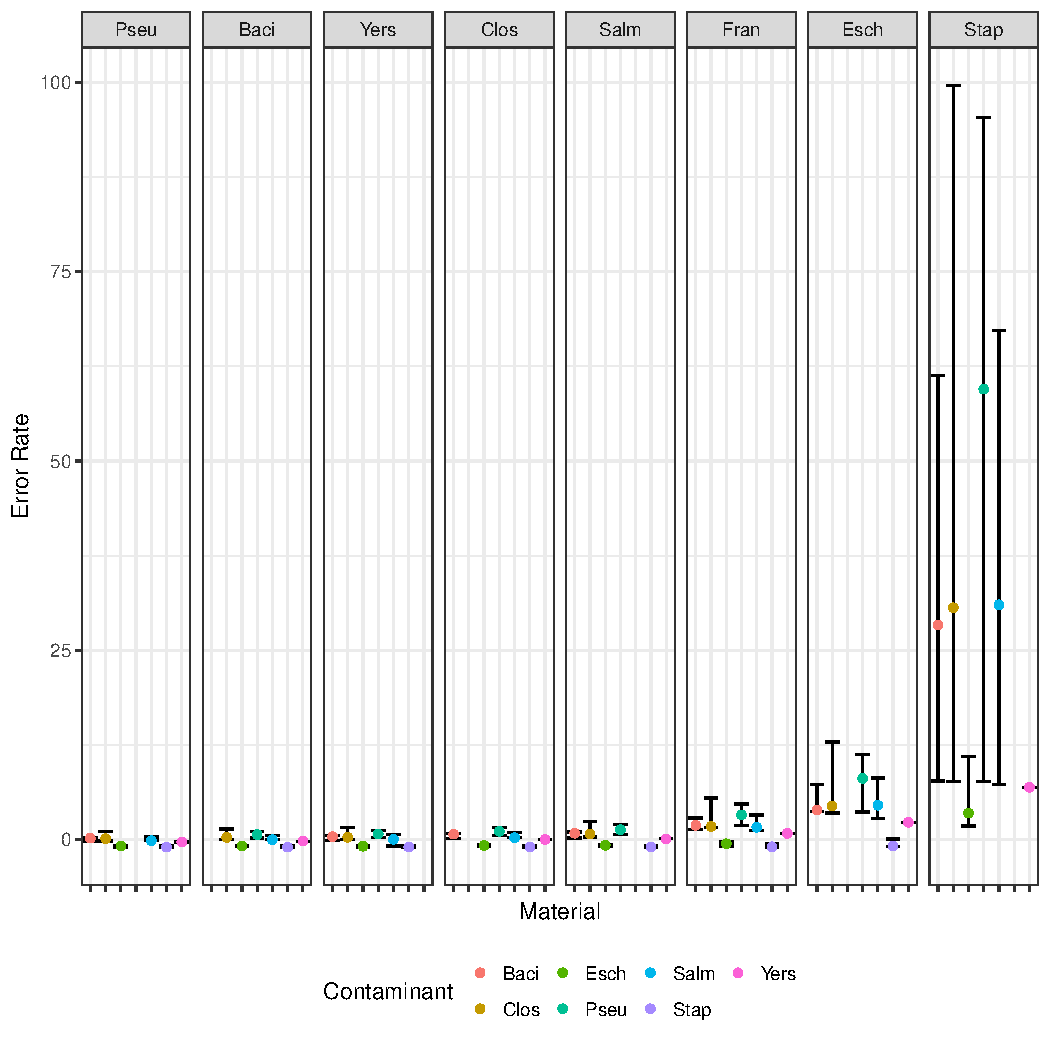
\includegraphics[width=\maxwidth]{figure/contam_resid-1} \caption[Total normalized residuals for pairwise combinations of material and contaminants]{Total normalized residuals for pairwise combinations of material and contaminants.}\label{fig:contam_resid}
\end{figure}


\end{knitrout}

The quantitative accuracy of contaminant proportions estimated by Pathoscope varied by material and contaminant strain.
The Pearson's correlation coeficient was used to measure the correlation between the estimated contaminant and true contaminant proportions. 
The estimated and true proportions were strongly correlated for all pairwise comparisons, with an overall median and 95\% confidence interval of 0.99945 (0.96943 - 0.99999 (Fig. \ref{fig:contam_fig}). 
Eight of the pairwise comparisons have correlation coefficients below 0.99, all of which have \textit{S. aureus} as either the contaminant or the material strain. 
Two coefficients were below 0.98, \textit{S. aureus} contaminated with \textit{P. aeruginosa} and \textit{S. enterica}, 0.952 and 0.969 respectively. 
Normalized contamiant proportion residuals, $(estimated-true)/true$, was used to assess the accuracy of the Pathoscope contaminant proportion estimates (Fig. \ref{fig:contam_resid}). 
The material genome strongly influenced the total normalized residuals with \textit{E. coli} and \textit{S. aureus} having consistently higher total normalized residuals compared to the other genomes. 


\section*{Discussion}

We demonstrated the potential for using the taxonomic sequence classification algorithm \textit{Pathoscope} to detect genomic contaminants in microbial materials using whole genome sequencing data. 
Using simulated sequencing data generated from individual genomes we provided a baseline assemement of the method to characterize the types of false postive contaminants identified the method. 
The false positive contaminants were split into three types; taxonomic ambiguities, phage, and method artifacts. 
We then characterized how contaminant detection veried by the material organism, the contaminant strain, and level of contamination. 
Overall the method was able to identify contaminant proportions at $10 \times 10^-3$ for most pairwise contaminant/material combinations. 
However, the accuracy of the estimated proportion of the contaminant in the simulated contaminated material varied by contaminant and material strain. 

The primary limitation of the proposed method are the observed false positive contamiants for single genome simulated sequencing data. 
Performing a baseline assement of false positive contaminant using simulated sequence data from the microbial material's genome sequence, and choosing the appropriate database and taxonomic assignment algorithm can help reduce the impact of false positive on the method's ability to identify organismal contmainants. 
Additionally, false positive contaminants are likely database and taxonomic assignment algorithm dependent. 
Removing sequences from the database for irrelevant contaminants, such as phage, plasmids, vectors, and multicellular eukaryotes can help reduce the proportion of false positives. 
Though the relevance of these contaminants is application specific. 
Similarly, using a curated database free of missclassified and unclassified sequence data would further help to reduce the proportion of false positive contaminants. 
Differentiating between two organisms with highly similar sequences will vary by taxonomic classification algorithm. 
Pathoscope was used for this proof of concept study as the method uses the full reads and paired end information for taxonomic classification rather then shorter sequence fragment, $k$-mers. 
Our assumption is that the longer sequence allows for better discrimination between highly simillar sequences. 
As there are numerous taxonomic classification algorithms, evaluating multiple methods using sequence data simulated from the material genome of interest can help to determine the optimal comtainant detection method for a specific microbial material. 

The ability to identify contaminants present at low concentrations is critical for when the material will be used for high sensitivity assays such as PCR. 
The minimum contaminant proportion was consistent for most simulated contaminant datasets, \textit{Yersinia} was only detected at a proportion of 0.1. 
The quantitative accuracy of the method varied by material and contaminant, but for all material-contaminant pairs, the Pathoscope estimated and true contaminant proportions were highly correlated. 
While not necessarily relevant to organismal contaminant detection, quantitative accuracy is relevant if the contaminant proportion is included in the report of analysis characterizing a material \citep{olson2016pepr}.  
Similar to the false positive contaminant baseline assessment. 
Similated data can be used to evaluate the minimal detectable contamiant proportion for specific contaminants of interest using different taxonomic assignment algorithms and databases. 
Additionally, sequencing at a higher depth would theoretically result in lower minimum detectable contaminant proportions and potentially increased quantitative accuracy due to the larger sample size (number of sequences).

\section*{Conclusions}
With the constant decline in the cost of sequencing, advances in sequence analysis methods, whole genome sequencing combined with a taxonomic assignment algorithm provide a viable alternative to commonly used organismal contaminant dection methods such as culturing, microscopy, and PCR. 
The method is suitable for detecting organismal contaminants in both genomic DNA and whole cell microbial materials without requiring any \textit{a priori} assumptions about the contaminant. 
Furthermore, the method was shown to detect contaminants making up $10 \times 10^{-3}$ proportion of cells in a high-throughput manner. 
Finally, the sequence data generated for organismal contaminant detection can be used to further characterize the material's genome and potentially identify other characteristics of interest such as the presence of virulence or antibotic resistence genes. 

\newpage

\section*{Acknowledgments}

The authors would like to thanks Dr. Steven Lund for his assistance in developing the study.
The Department of Homeland Security (DHS) Science and Technology Directorate supported this work under the Interagency Agreement HSHQPM-12-X-00078 with the National Institute of Standards and Technology (NIST).
Opinions expressed in this paper are the authors’ and do not necessarily reflect the policies and views of DHS,  NIST, or affiliated venues.
Certain commercial equipment, instruments, or materials are identified in this paper in order to specify the experimental procedure adequately.
Such identification is not intended to imply recommendations or endorsement by NIST,
nor is it intended to imply that the materials or equipment identified are necessarily the best available for the purpose.
Official contribution of NIST; not subject to copyrights in USA.

\bibliography{genomic_purity}

\end{document}
